\chapter{Eksperymenty numeryczne}
\label{cha:numeryczne}
nieaddytywne? testy? \par
W celu przeprowadzenia eksperymentów numerycznych zaimplementowano rozszerzony filtr Kalmana oraz filtr Kalmana Gaussa-Hermite'a. Implementację przeprowadzono w~języku Python z~wykorzystaniem otwartoźródłowej biblioteki NumPy, przeznaczonej do~szybkiego wykonywania obliczeń macierzowych. Interfejs wykonanych modułów został stworzony zgodnie z~paradygmatem programowania obiektowego. \par
Funkcje teoretyczne: 2 funkcje Liu, moje funkcje: rmse jako funkcja parametru a funkcji, EKF, GHKF-2, GHKF-3, GHKF-5?, czasy działania algorytmów, 2 warianty: model procesu lub model pomiarów nieliniowy, 2 wymiary \par
Do~porównania działania filtrów użyto początkowo dyskretnego nieliniowego modelu systemu dynamicznego, wykorzystywanego wcześniej w~\cite{Liu} i~\cite{Germani}. Przeprowadzono 50 iteracji dla czasów 1-50 i~wykorzystano EKF oraz GHKF trzeciego stopnia do~estymacji stanu systemów.\par
Model systemu wyglądał następująco:
\begin{align}\label{eq:LiuModel1}
	&\left\{ 
	\begin{array}{l}
	x_1(t+1) = 0.8x_1(t) + x_1(t)x2(t) + 0.1 + 0.01w_1(t) \\
	x_2(t+1) = 1.5x_2(t) - x_1(t)x_2(t) + 0.1 + 0.01w_1(t) \\
	\end{array}
	\right.\nonumber \\
	&\left\{ 
	\begin{array}{l}
	z_1(t+1) = x_1(t+1) + 0.04v_1(t+1) \\
	z_2(t+1) = x_1(t+1) + 0.04v_2(t+1)
	\end{array}
	\right.
\end{align}
gdzie szum procesu oraz szum pomiaru są nieskorelowanymi białymi szumami gaussowskimi z~następującymi rozkładami: $\boldsymbol{w}(t) \sim \mathcal{N}(\boldsymbol{0}, \boldsymbol{Q})$, $\boldsymbol{v}(t) \sim \mathcal{N}(\boldsymbol{0}, \boldsymbol{R})$, $\boldsymbol{Q}=diag(0.1, 0.2)$, $\boldsymbol{R}=diag(0.1, 0.2)$; początkowy stan systemu to: $\boldsymbol{x}(0) = [1,1]^T$, $\boldsymbol{P}(0|0) = \boldsymbol{I}_{2 \times 2}$.\\ 
Jako miarę skuteczności filtracji użyto pierwiastka z~błędu średniokwadratowego (ang. \textit{root-mean-square error}, RMSE), który dla $T$ estymat $\hat{x}_t$ rzeczywistych wartości $x_t$ jest definiowany następująco:
\begin{align}\label{eq:rmse}
\text{RMSE} = \sqrt{\frac{\sum_{t=1}^{T}(\hat{x}_t - x_t)^2}{T}}
\end{align}
Wykorzystanie EKF wymagało obliczenia macierzy $\boldsymbol{G}$ i $\boldsymbol{H}$:
\begin{align}\label{eq:LiuModel1GH}
\boldsymbol{G}&=
\begin{bmatrix}
x_2 + 0.8 & x_1 \\
-x_2 & 1.5 - x_1
\end{bmatrix} \nonumber \\
\boldsymbol{H}&=\boldsymbol{I}_{2 \times 2}
\end{align}
Dla EKF wartość RMSE wyniosła, odpowiednio dla $x_1$ i~$x_2$, 0.01244 i~0.01042, natomiast dla GHKF 0.01246 oraz 0.00961. Rysunek \ref{fig:Liu1_errors} przedstawia wykresy różnic pomiędzy wartością estymowaną, a~rzeczywistą dla zmiennych stanu badanego systemu. Oba algorytmy dobrze poradziły sobie z~postawionym problemem, wartości błędów były bardzo niewielkie, a~różnice między wartościami wyjściowymi algorytmów minimalne.   
\begin{figure}
	\centering
	\begin{subfigure}[b]{0.4\linewidth}
		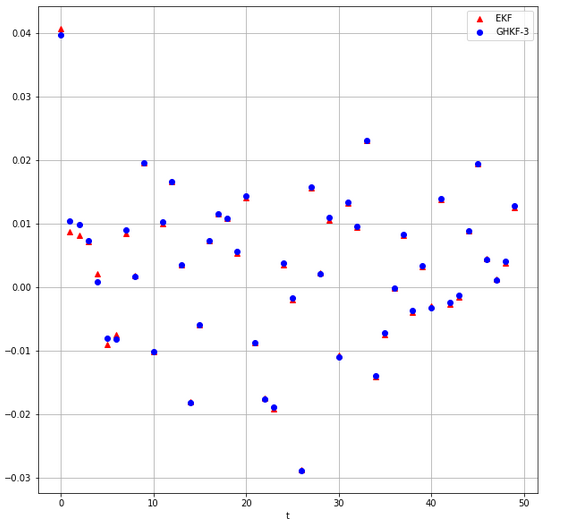
\includegraphics[width=\linewidth]{Liu1_x1_error.png}
		\caption{}
		\label{fig:Liu1_errors_a}
	\end{subfigure}
	\begin{subfigure}[b]{0.4\linewidth}
		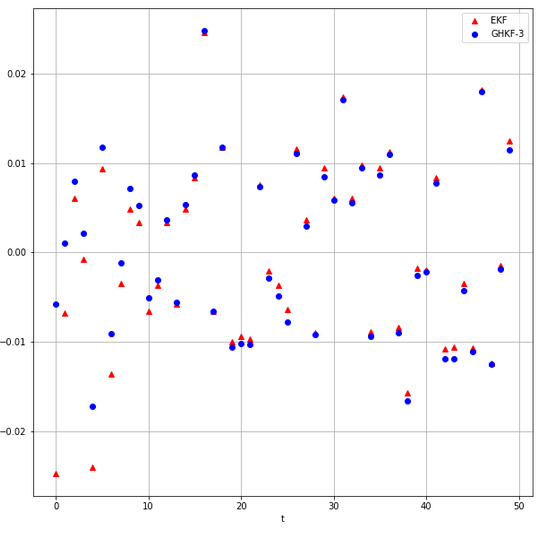
\includegraphics[width=\linewidth]{Liu1_x2_error.png}
		\caption{}
		\label{fig:Liu1_errors_b}
	\end{subfigure}
	\caption{Różnice między wartością estymowaną, a rzeczywistą dla $x_1$(\ref{fig:Liu1_errors_a}) oraz $x_2$ (\ref{fig:Liu1_errors_b}).}
	\label{fig:Liu1_errors}
\end{figure}


\par


W~celu zbadania, jak nieliniowość funkcji wpływa na~działanie obu rodzajów filtrów, przeprowadzono 

Problemy praktyczne:  śledzenie pocisku balistycznego, dwuwymiarowe śledzenie ruchu obiektu, śledzenie wyłącznie z wykorzystaniem namiaru 